%%%%%%%%%%%%%%%%%%%%%%%%%%%%%%%%%%%%%%%%%%%%%%%%%%%%%%%%%%%%%%%%%%%%%%%%
%                                                                      %
%     File: Thesis_Background.tex                                      %
%     Tex Master: Thesis.tex                                           %
%                                                                      %
%     Author: Andre C. Marta                                           %
%     Last modified : 29 Jun 2022                                      %
%                                                                      %
%%%%%%%%%%%%%%%%%%%%%%%%%%%%%%%%%%%%%%%%%%%%%%%%%%%%%%%%%%%%%%%%%%%%%%%%

\chapter{Protocolo PTP}
\label{chapter:background}

O PTP é um protocolo de sincronização temporal inicialmente introduzido pela norma IEEE 1588. Atualmente, a versão que vem sendo mais adotada pela indústria é a versão IEEE 1588:2008, vulgarmente identificada como IEEE 1588V2, atualizada em 2020 \cite{PTP}.
A referida atualização do protocolo trouxe melhorias relativas à versão inicial como o mecanismo \textit{Peer-to-Peer} e o modo \textit{Transparent Clock} que serão posteriormente explicadas. 


%%%%%%%%%%%%%%%%%%%%%%%%%%%%%%%%%%%%%%%%%%%%%%%%%%%%%%%%%%%%%%%%%%%%%%%%
\section{Conceitos fundamentais}
\label{section:overview}

A execução do protocolo decorre sobre uma estrutura hierárquica \textit{Master}-\textit{Slave} implementada sobre um meio de comunicação. A rede será constituída por um, ou mais, dispositivos denominados de \textit{Clocks} com suporte para a execução do algoritmo e portadores de relógios internos chamados de \textit{Local Clocks}. Os vários canais de comunicação de um \textit{Clock}, ou portos, são agrupados em instâncias. A integridade da rede é dividida logicamente em domínios, na qual as várias instâncias de um domínio se sincronizam entre si.  Durante a execução contínua do protocolo, as instâncias pertencentes a dispositivos com \textit{Local Clocks} de menor precisão sincronizam-se com as instâncias pertencentes a dispositivos com \textit{Local Clocks} de maior precisão. \par  A instância que está no topo da hierarquia, portadora do \textit{Local Clock} de maior precisão, e à qual todas as restantes instâncias se sincronizam direta ou indiretamente, é denominada de \textit{GrandMaster} e normalmente pertence a um dispositivo que possui um recetor GPS. As várias instâncias de um domínio possuem uma estimativa do tempo no \textit{Grandmaster}, denominada \textit{Local PTP Clock}, que é o elemento de sincronização. Quando uma instância sincroniza o seu \textit{Local PTP Clock} com outra, esta funciona como \textit{Slave} para a segunda, que por sua vez funciona como \textit{Master}.

Os vários tipos de instâncias presentes na norma, que podem fazer parte da rede de comunicação, são os seguidamente referidos. 

\begin{itemize}
  \item \textit{Ordinary Clock}  - \quad Instância que apenas possui um porto no domínio. Pode funcionar como \textit{Slave} ou \textit{Master}. Quando em modo \textit{Slave} deve sincronizar-se com um dos \textit{Masters} presentes na rede. Num sistema de automação
  de subestações será o caso das relés de proteção ou dos sistemas SCADA, posteriormente explicados. 
  Quando em modo \textit{Master}, serve como referência temporal para um conjunto de \textit{Slaves} que se encontrem numa posição inferior na hierarquia.
  \item \textit{Boundary Clock}  - \quad Instância com múltiplos portos no domínio, que atua como \textit{Master} para determinado conjunto de instâncias e como \textit{Slave} para outras.
  \item \textit{Transparent Clock} - \quad Introduzido na norma IEEE1588V2. Transmite os sinais de sincronização na rede. É a instância vulgarmente em funcionamento nos comutadores de \textit{Ethernet}, podendo funcionar em modo P2P (\textit{Peer-to-Peer}) ou E2E (\textit{End-to-End}) consoante o modo de atuação.
\end{itemize}

Além das referidas instâncias, a rede pode ainda incluir dispositivos não relacionados ao protocolo e \textit{Management Nodes} responsáveis por transmitir à rede mensagens portadoras de informação relativa à configuração da execução do protocolo. \par
A figura 2.1 representa um exemplo simples de uma rede hierárquica do \textit{tipo Master-Slave}.

\begin{figure}[!htb]
  \centering
  \includegraphics[width=1\textwidth]{Figures/sss.jpg}
  \caption[Hierarquia \textit{Master-Slave} no PTP]{Hierarquia \textit{Master-Slave} no PTP (fonte: \cite{PTP2019})}
  \label{fig:airbus1}
\end{figure}


O modelo de rede apresentado é constituido por 6 instâncias: dois \textit{Boundary Clocks} e quatro \textit{Ordinary Clocks}. No exemplo, o \textit{Ordinary Clock}-1 possui o \textit{Local Clock} de maior precisão e é a raiz da rede, atuando como \textit{Grandmaster}. As restantes instâncias do tipo \textit{Ordinary Clock} relegam-se assim ao papel de \textit{Slave}. Os diferentes portos dos \textit{Boundary Clocks} desempenham o papel de \textit{Master} ou \textit{Slave} consoante a posição em que se encontrem na hierarquia. No exemplo, o porto 1 de \textit{Boundary Clock}-1 é um \textit{Slave} para o \textit{Grandmaster}, enquanto os restantes portos atuam como \textit{Masters}. Relativamente ao \textit{Boundary Clock}-2, o porto 1 é \textit{Slave} relativamente a \textit{Boundary Clock}-1, enquanto os restantes portos atuam como \textit{Masters} para os respetivos \textit{Ordinary Clocks}. Os cinco diferentes caminhos entre as várias instâncias podem ainda incluir vários \textit{Transparent Clocks}. Essas instâncias participam ativamente na correta execução do PTP, no entanto, não fazem parte da hierarquia \textit{Master}-\textit{Slave}. \par

\section{Algoritmo \textit{Best Master Clock}}
\label{section:overview}

Por diversos motivos, pode ser necessário, ou desejável, alterar a hierarquia ou estrutura, da rede de comunicação. Isso pode acontecer por alterações dos atributos dos diferentes \textit{Clocks} presentes, por avarias, adição de novos dispositivos ou alterações na topologia da rede. Assim, em paralelo com todas as operações necessárias para a sincronização dos múltiplos \textit{Clocks}, decorre também a execução do algoritmo BMC (\textit{Best Master Clock}), com o objetivo de manter constantemente uma hierarquia \textit{Master}-\textit{Slave} óptima. O BMC é um algoritmo executado individualmente em cada porto de \textit{Boundary Clocks} e \textit{Ordinary Clocks} e encontra-se dividido em duas partes.\par Primeiramente, os diversos portos de uma instância comparam as características do seu \textit{Local Clock} com as características dos vários \textit{Local Clocks} dos quais cada porto tem conhecimento. A informação sobre as características dos \textit{Local Clocks}, juntamente com informação sobre as respestivas instâncias, é transmitida através de mensagens do tipo \textit{Announce}, com uma periodicidade predefinida. De forma a escolher qual de entre dois \textit{Local Clocks} é o melhor são comparadas diversas características, tais como a precisão, a variância e a classe.  \par
Finalizada a primeira metade da iteração do algoritmo, e identificados os melhores \textit{Local Clocks} a concorrer para \textit{Master} dos vários portos e o melhor de entre eles, cada porto fica responsável por individualmente decidir qual o seu modo de operação, até que seja finalizada a seguinte iteração do algoritmo. Um porto pode ficar num de três estados possíveis: \textit{Master}, \textit{Slave} ou \textit{Passive}. Um porto fica em estado de \textit{Slave} quando a mensagem \textit{Announce} com a informação sobre o melhor \textit{Local Clock} for recebida no respetivo porto.
Se a referida mensagem \textit{Announce} for recebida noutro porto, este pode ficar no estado \textit{Passive} ou \textit{Master}. Se o melhor \textit{Local Clock} cuja mensagem \textit{Announce} foi recebida no respetivo porto for topologicamente superior ao melhor \textit{Local Clock} do qual a instância tomou conhecimento, o porto fica no estado \textit{Passive}, continuando a receber mensagens \textit{Announce}, mas sem desempenhar funções de sincronização. Caso contrario, o porto fica no estado \textit{Master}. A comparação topológica consiste em analisar atributos não diretamente relacionados ao desempenho dos \textit{Local Clocks}, tais como parâmetros de identificação dos portos e a quantidade de \textit{Clocks} entre as instâncias. O porto pode ainda ficar no estado \textit{Master}, quando o próprio \textit{Local Clock} da instância é o melhor de entre todos aqueles que foram comparados na primeira parte do algoritmo, situação que faz deste o \textit{GrandMaster} da rede.

\section{Aplicação}
\label{section:theory1}


A execução do PTP é conseguida através da troca de diferentes tipos de mensagens padronizadas, portadoras da informação necessária para se atingir o objetivo de sincronização dos vários \textit{Clocks}. O formato das mensagens consiste num cabeçalho, corpo da mensagem e sufixo. O cabeçalho é comum a todas as mensagens e tem o tamanho de 34 octetos. Contrariamente, o corpo muda consoante o tipo de mensagem. O sufixo, quando existe, é constituído por um conjunto de estruturas de dados do tipo TLV (\textit{Type-Length-Value}).\par As mensagens estão dividias em duas classes: evento e geral. As mensagens da classe evento diferem da classe geral por requererem o registo, com uma margem de erro dada pela incerteza da medição nos dispositivos, do instante de tempo de envio da mensagem na sua origem e da recepção no destinatário. As mensagens pertencentes à classe evento são as seguintes:

\begin{itemize}
  \item \textit{Sync}  - \quad Mensagem transmitida pelos \textit{Masters} para sincronização dos \textit{Slaves}.
  \item \textit{Delay\_Req}  - \quad Mensagem enviada por um \textit{Slave} para um \textit{Master} ao qual se sincroniza, para iniciar o processo de cálculo do tempo de propagação de uma mensagem entre ambos. 
  \item \textit{PDelay\_Req}  - \quad Mensagem enviada por uma instância que suporta o mecanismo P2P para as instâncias vizinhas com igual suporte deste mecanismo.
  \item \textit{PDelay\_Resp} - \quad Mensagem enviada como resposta à mensagem do tipo \textit{PDelay\_Req} 
\end{itemize}


As mensagens pertencentes à classe geral são as seguintes:

\begin{itemize}
  \item \textit{Announce}  - \quad Mensagens que transmitem a informação relativa às características dos diferentes \textit{Clocks} na rede a concorrer pelas posições de \textit{Master}, durante a execução do algoritmo BMC.
  \item \textit{Follow\_Up}  - \quad  Mensagem enviada pelos \textit{Master} que contém o instante de transmissão de uma mensagem \textit{Sync}. É enviada quando um \textit{Master} ou um \textit{Transparent Clock} intermédio não possui \textit{hardware} capaz de registar numa mensagem o instante de transmissão da mesma.
  \item \textit{Delay\_Resp}  - \quad Mensagem que envia para o \textit{Slave} qual o instante de recepção no \textit{Master} da correspondente mensagem do tipo \textit{Delay\_Request}.
  \item \textit{Pdelay\_Resp\_Follow\_Up} - \quad Mensagem enviada por uma instância que contém o instante de tempo de transmissão de uma mensagem \textit{PDelay\_Resp}. É enviada quando a instância geradora da mensagem \textit{PDelay\_Resp} não possui \textit{hardware} capaz de registar numa mensagem o instante de transmissão da mesma.
  \item \textit{Management} -\quad Mensagem que transmite informação relativa às configurações do protocolo.
  \item \textit{Signaling} -\quad Mensagem que transmite informação relativa às várias instâncias do PTP.  
\end{itemize}


Através da realização de cálculos simples sobre os instantes de envio e recepção das mensagens da classe evento, as instâncias em modo \textit{Slave} conseguem calcular o desfasamento entre o seu \textit{Local PTP Clock} e o \textit{Local PTP Clock} de um \textit{Master}, denominado na norma como \textit{offsetFromMaster}. A sincronização com o \textit{Master} obtém-se minimizando o valor do \textit{offsetFromMaster}, recorrendo a meios não definidos na norma. A comunicação dos referidos instantes de tempo pode ser conseguida exclusivamente com as mensagens \textit{Sync}, \textit{Delay\_Req}, \textit{Delay\_Resp} e, quando há suporte para tal, \textit{PDelay\_Req e PDelay\_Resp}. Esse modo de operação do PTP é denominado de PTP \textit{One-Way}. De forma a evitar as mensagens \textit{Follow\_Up} e \textit{PDelay\_Resp\_Follow\_Up} é necessário \textit{hardware} mais sofisticado, capaz de registar o instante em que começa a transmição de uma mensagem e alterar a referida mensagem antes de finalizado o envio através de um porto. O referido modo de operação exclui assim que a elaboração integral dos algoritmos para execução do PTP seja efectuada em \textit{software}. A vantagem da operação \textit{One-Way} é reduzir a quantidade de tráfego na rede necessário para executar o protocolo. Quando o \textit{hardware} dos dispositivos presentes não permite a execução \textit{One-Way}, é necessário o envio das mensagens \textit{Follow\_Up} e \textit{PDelay\_Resp\_Follow\_Up} para informar os \textit{Slaves} de qual o instante exato de transmissão das mensagens \textit{Sync} e \textit{Delay\_Resp}. Denomina-se o modo de operação PTP \textit{Two-Way}.   \par
O cálculo do \textit{offsetFromMaster} ocorre de cada vez que um \textit{Slave} recebe uma mensagem \textit{Sync} ou, se o modo de funcionamento for \textit{Two-Way}, a respetiva mensagem \textit{Follow\_up}. Para um correto cálculo do \textit{offsetFromMaster} o \textit{Slave} precisa de calcular previamente o atraso de propagação de uma mensagem entre si e o \textit{Master}, o que pode ser feito recorrendo ao mecanismo E2E ou P2P.

\subsection{Mecanismo \textit{End-to-End}}

Na versão inicial do PTP o atraso de caminho entre um \textit{Master} e um \textit{Slave} era exclusivamente calculado com o mecanismo E2E. Uma execução do referido mecanismo está demonstrada na figura 2.2. No exemplo é assumido que o \textit{Slave} está adiantado 8 $\mu$s em relação ao \textit{Master} com o qual se sincroniza, e que há um atraso de caminho de  6 $\mu$s em ambos os sentidos. Na figura são destacados os seguintes instantes de tempo: 


\begin{itemize}
  \item T1  - \quad Instante de tempo de transmissão da mensagem \textit{Sync} pelo \textit{Master}.
  \item T2  - \quad Instante de tempo de recepção da mensagem \textit{Sync} pelo \textit{Slave}. 
  \item T3  - \quad Instante de tempo de transmissão da mensagem \textit{Delay\_Req} pelo \textit{Slave}.
  \item T4 - \quad Instante de tempo de recepção da mensagem \textit{Delay\_Req} pelo \textit{Master}.
\end{itemize}

Se se assumir que o tempo que uma mensagem demora a deslocar-se entre o \textit{Master} e o \textit{Slave} é constante e igual nos dois sentidos, o atraso de caminho entre o \textit{Master} e o \textit{Slave} e o \textit{offsetFromMaster} são calculados através das equações 2.1 e 2.2.

\begin{equation}
 Atraso =  \dfrac{(T4 - T1) - (T3 - T2)}{2}   
\end{equation}
 
\begin{equation}
   offsetFromMaster =  T2 - T1 - Atraso   
\end{equation}



\begin{figure}[!htb]
  \centering
  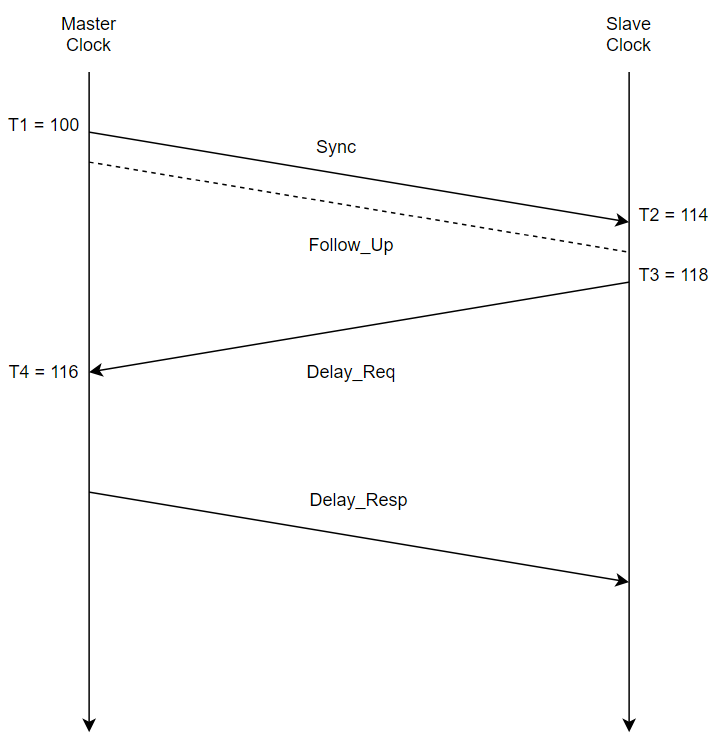
\includegraphics[width=0.8\textwidth]{First.png}
  \caption[Mecanismo E2E]{Mecanismo E2E}
  \label{fig:airbus1}
\end{figure}


Inserindo na equação 2.2 os valores dos tempos de envio e recepção das mensagens que estão definidos na figura, comprova-se o valor de 6 $\mu$s para o atraso no caminho. 

\[ Atraso =  \dfrac{(T4 - T1) - (T3 - T2)}{2} = \dfrac{(116 - 100) - (118 - 114)}{2} = 6\]

 Este procedimento para o cálculo do \textit{offsetFromMaster} formulado na versão inicial do PTP funciona com muito precisão quando o tempo de propagção da mensagen é igual nos dois sentidos, no entanto, incorre no problema causado pela presença de dispositivos intermédios já mencionado no capítulo introdutório.. Por exemplo, se houver congestionamento num dispositivo intermédio entre o \textit{Slave} e o \textit{Master} no momento em que por ele transita a mensagem \textit{Delay\_Req}, a mesma terá um tempo de propagação mais elevado do que a mensagem \textit{Sync}. Consequentemente, o atraso será erradamente calculado com a fórmula previamente apresentada, assim como os \textit{Local Clocks} serão imprecisamente sincronizados. Da mesma forma, o desfasamento entre o \textit{Master} e o \textit{Slave} também não será corretamente calculado se a mensagem \textit{Sync} for forçada a um atraso de propagação diferente daquele que foi previamente calculado com o mecanismo E2E. Para calcular corretamente os atrasos, o tempo de residência das mensagens nos dispositivos intermédios teria que ser registado e comunicado ao \textit{Slave}. As manipulações ás mensagens a efectuar pelos dispositivos intermédios para comunicar o tempo de residências das mensagens foram introduzidas no PTPV2. Ainda que as manipulações tenham alguns detalhes adicionais, em traços básicos, o tempo de residência nos \textit{Transparent Clocks} é adicionado ao campo \textit{correctionField} das mensagens e posteriormente subtraído pelo \textit{Slave} nos cálculos do atraso e \textit{offstedFromMaster}, obtendo-se as equações 2.3 e 2.4. 

\begin{equation}
    Atraso =  \dfrac{(T4 - T1) - (T3 - T2) - ResidenceTimeSync - 
    ResidenceTimeDelay\_Req}{2}
\end{equation}

\begin{equation}
    offsetFromMaster =  T2 - T1 - Atraso - ResidenceTimeSync
\end{equation}

Na figura 2.3 é apresentado um exemplo de como a implementação do suporte para funcionamento como \textit{Transparent Clcok} em dois dispositivos intermédios é usado para corrigir as assimetrias no tempo de propagação causadas por tempos de residência variáveis.


\begin{figure}[!htb]
  \centering
  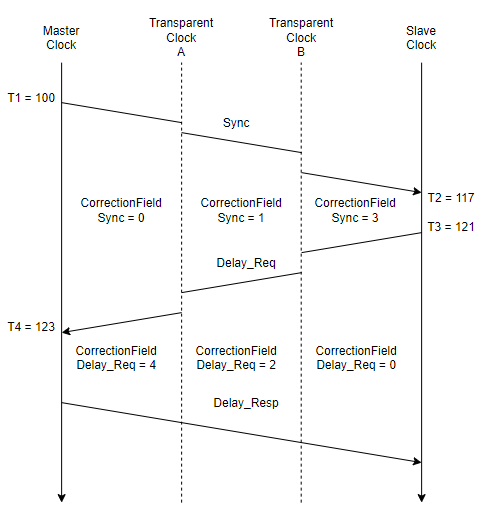
\includegraphics[width=0.8\textwidth]{correction.png}
  \caption[Aplicação do \textit{Transparent Clock}]{Aplicação do \textit{Transparent Clock}}
  \label{fig:airbus1}
\end{figure}


O exemplo é semelhante ao anterior, mas são descriminados dois \textit{Transparent Clocks} atravessados pelas várias mensagens que transitam entre o \textit{Slave} e o \textit{Master}. Além disso, é assumido que a mensagem \textit{Sync} é retardada por 1 $\mu$s no \textit{Transparent Clock} A e por 2 $\mu$s no \textit{Transparent Clock} B, e que a mensagem do tipo Delay\_Req demora 2 $\mu$s em cada um dos \textit{Transparent Clocks}. Como tal, é totalizado um valor de 3 $\mu$s para o \textit{CorrectionField} da mensagem \textit{Sync} quando esta chega ao \textit{Slave}, e de 4 $\mu$s para a mensagem \textit{Delay\_Req} quando esta chega ao \textit{Master}. 
Tal como no exemplo anterior, é assumido um desfasamento de 8 $\mu$s entre os \textit{Local PTP Clocks} e um tempo de propagação de 6 $\mu$s, e são apresentados os tempos de envio e recepção das mensagens \textit{Sync} e \textit{Delay\_Req}. Substituindo na equação 2.4 os instantes de tempo presentes no exemplo 
e os valores do \textit{CorrectionField} explicados, obtém-se o atraso de 6$\mu$s assumido.

\[ Atraso = \dfrac{(123 - 100) - (121 - 117) - 3 - 4}{2} = 6\]

\subsection{Mecanismo \textit{Peer-to-Peer}}

Alternativamente pode ser usado o mecanismo P2P para proceder à sincronização dos \textit{Local PTP Clocks}. Nesta variante, todos os dispositivos que participam na sincronização entre um \textit{Master} e um \textit{Slave} mantêm a informação do tempo de propagação de uma mensagem entre si e os seus vizinhos. Quando uma mensagem \textit{Sync} é enviada pelo \textit{Master}, todos os dispositivos intermédios adicionam ao \textit{CorrectionFieldSync} o tempo de residência no dispositivo e o tempo de propagação entre o dispositivo imediatamente anterior no caminho e si mesmo. Assim, quando a mensagem \textit{Sync} ou a respectiva mensagem \textit{Follow\_up} chegam ao \textit{Slave}, o atraso de propagação entre o \textit{Master} e o dispositivo imediatamente antes do \textit{Slave}, e todos os tempos de residência, já se encontram totalizados no \textit{CorrectionField}. Assím, para obter o \textit{Slave} obter o atraso entre si e o \textit{Master}, este apenas precisa de somar o atraso entre si e o seu vininho ao somatório dos restantes atrasos totalizados no \textit{correctionField} da mensagem \textit{Sync}. \par 
Por forma a obter os tempos de propagação entre dois vizinhos são trocadas mensagens do tipo \textit{PDelay\_Req}, \textit{PDelay\_Resp} e \textit{PDelay\_Resp\_Follow\_Up}. Um exemplo de cálculo do atraso de caminho está demonstrado na figura 2.4. Os valores do tempo de propagação e do desfasamento são os mesmos dos exemplos anteriores. 


No figura estão indicados os seguintes instantes de tempo:

\begin{itemize}
  \item T1  - \quad Instante de tempo de transmissão da mensagem \textit{PDelay\_Req} pelo \textit{Transparent Clock} A.
  \item T2  - \quad Instante de tempo de recepção da mensagem \textit{PDelay\_Req} pelo \textit{Transparent Clock} B. 
  \item T3  - \quad Instante de tempo de transmissão da mensagem \textit{PDelay\_Resp} pelo \textit{Transparent Clock} B.
  \item T4 - \quad Instante de tempo de recepção da mensagem \textit{PDelay\_Resp} pelo \textit{Transparent Clock} A.
\end{itemize}

O valor do atraso de caminho é obtido recorrendo à equeação 2.6:

\begin{equation}
    Atraso =  \dfrac{(T4 - T1) - (T3 - T2)}{2}
\end{equation}



Substituindo os instantes de tempo na equação 2.6, obtém-se 6 $\mu$s.

\[ Atraso =  \dfrac{(116 - 100) - (118 - 114)}{2} = 6\]

\begin{figure}[H]
  \centering
  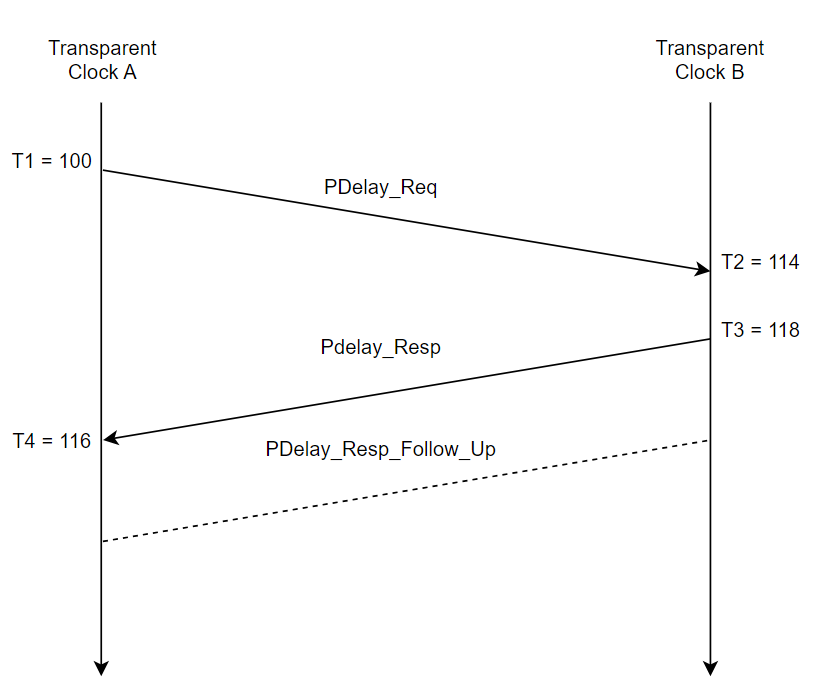
\includegraphics[width=0.8\textwidth]{Peed.png}
  \caption[Mecanismo P2P]{Mecanismo P2P}
  \label{fig:airbus1}
\end{figure}

\section{\textit{Power Utility Profile}}
\label{section:theory1}



O PTP pode ser implementado em redes construídas para funções variadas com diversos requisitos de desempenho.  Por forma a ajustar o PTP da melhor forma possível às características da rede na qual se recorre ao algoritmo, a norma dá liberdade a organizações relevantes em várias indústrias para que estas definam restrições a nível dos atributos e funcionalidades do PTP, aquando da sua implementação na respetiva indústria. À compilação destas variadas restrições dá-se o nome de perfil. Um perfil deve definir quais as opções do BMC que devem ser implementas, a utilização do mecanismo E2E ou P2P, os vários mecanismos de configuração da execução do protocolo, mecanismos de transporte, precisão e incerteza requerida ao nível da sincronização dos \textit{Clocks}, gamas de valores permitidas para os vários atributos do PTP, e as instâncias do PTP permitidas, requeridas ou proibidas. \par 

\iffalse
Por forma a integrar componentes que possam ser provenientes de diferentes fabricantes, foi criada a norma IEC 61850 que define protocolos de comunicação para dispositivos inteligentes em sistemas de automação de subestações elétricas (SAS) \cite{SAS}. A norma divide o SAS em três níveis:

\begin{itemize}
  \item \textit{Process Level} - Nível onde é feita aquisição de dados referentes ao vários equipamentos e estruturas da subestação, posteriormente enviados para os níveis superiores. É aqui que se encontram as \textit{Merging Units} (MU) e as \textit{Phasor Measurement Units}. 
  \item \textit{Bay level} - Nível onde se encontram vários \textit{Intelligent Electronic Devices} (IED), responsáveis por controlar individualmente os vários equipamentos da subestação. Além disso, encontram-se também neste nível equipamentos de segurança, como as relés de proteção.
  \item \textit{Station level} - É o nível mais próximo dos operadores das SAS. Inclui os sistemas SCADA (\textit{Supervisory Control and Data Acquisition}), que consistem num conjunto de equipamentos de \textit{hardware} e \textit{software}, utilizados para controlar e monitorizar a subestação com recurso a dados capturados no primeiro nível. Os operadores interagem com os sistemas SCADA através das \textit{Human Machine Interfaces} (HMI).
\end{itemize}

A arquitetura típica de um SAS que segue as regras definidas na norma IEC 61850 está ilustrada na figura 2.5.

\begin{figure}[H]
  \centering
  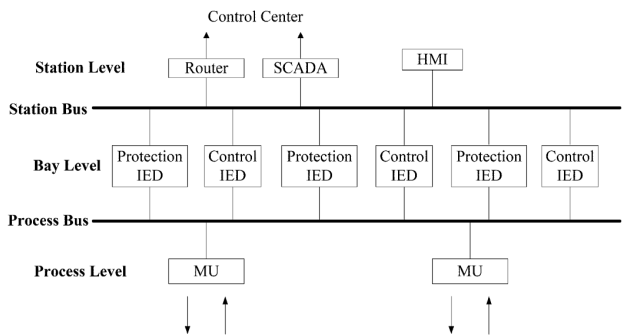
\includegraphics[width=1\textwidth]{SAS.png}
  \caption[Arquitetura típica de um sistema de automação de subestações elétricas ]{Arquitetura típica de um sistema de automação de subestações elétricas (fonte: \cite{comparison})}
  
  \label{fig:airbus1}
\end{figure}


\fi
Incluída na norma IEC 61850, a norma que define os protocolos de comunicação entre IEDs numa subestaçãoe elétrica, pode encontrar-se a subnorma IEEE 61850-9-3, vulgarmente denominada por \textit{Power Utility Profile} (PUP) \cite{PUP}, optimizada para fornecer a precisão de 1$\mu$s nas sincronizações, necessária para garantir a operacionalidade determinística dos sistemas críticos, sem inserir tráfego excessivo na rede e sem precisar de \textit{Boundary Clocks} excessivamente complexos.
O PUP exige que as comunicações sejam feitas sobre \textit{Ethernet}, com recurso exclusivamente ao mecanismo P2P e, preferencialmente, em modo de operação \textit{One-Way}, sem restrições ao nível do modo de operação do BMC. As mensagens usadas no protocolo devem recorrer sempre a tramas do tipo \textit{multicast}. Com a escolha do mecanismo P2P, o \textit{GrandMaster} da rede apenas comunica com o \textit{Transparent Clock} com o qual tem uma ligação. Assim, é possível aumentar a quantidade de dispositivos na rede a sincronizarem-se, em última instância, com o \textit{GrandMaster}, sem que para isso o mesmo precise de processar uma maior quantidade de tráfego. O PUP tem ainda a vantagem de ser compatível com protocolos que assegurem a resiliência da rede face a falhas singulares de elementos na mesma, tais como o \textit{Parallel Redundancy Protocol} (PRP) \cite{PRP}, e o \textit{High-availability Seamless Redundancy} (HSR) \cite{HSR}. Por forma a cumprir com a precisão de 1 $\mu$s, necessária em subestações elétricas, o PUP define as seguintes imprecisões máximas aceitáveis nos vários elementos na rede:  

\begin{itemize}
  \item \textit{GrandMaster Clock} - 250 ns
  \item \textit{Boundary Clock} - 200 ns
  \item \textit{Transparent Clock} - 50 ns
\end{itemize}

As imprecisões definidas permitem alcançar o desempenho requerido numa situação em que as mensagens tenham que atravessar até 15 \textit{Transparent Clocks} para se deslocarem do \textit{GrandMaster} com destino a um \textit{Slave}. O PUP exige ainda a transmissão periódica, com intervalos de 1 s, das mensagens do tipo \textit{Announce}, \textit{Sync} e \textit{PDelay\_Req}. As mensagens \textit{Announce} devem ser descartadas quando circulam por mais de 3 s na rede. 

\iffalse

\par Na figura 2.6 encontra-se ilustrado um exemplo de uma rede onde um \textit{switch} de \textit{Ethernet} é usado como \textit{Transparent Clock} para contribuir para a sincronização dos vários elementos de uma SAS com um \textit{Grandmaster}.

\begin{figure}[H]
  \centering
  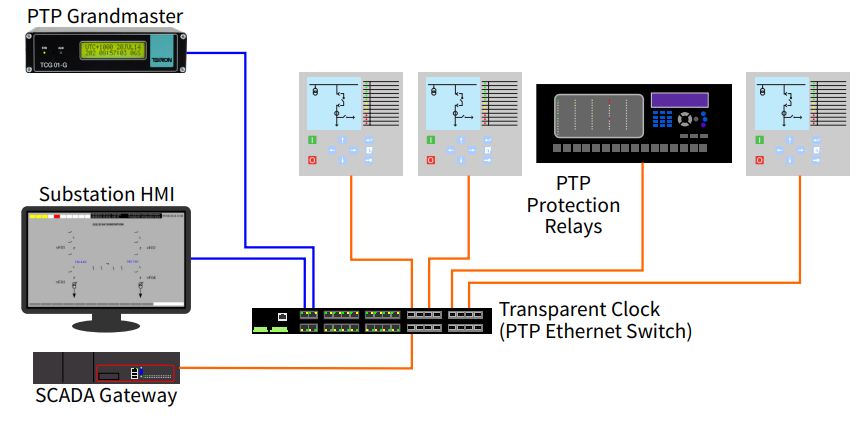
\includegraphics[width=1\textwidth]{topology.png}
  \caption[Rede numa SAS sincronizada via PTP ]{Rede numa SAS sincronizada via PTP (fonte: \cite{Electrical})}
  \label{fig:airbus1}
\end{figure}

\fi

\section{Implementação de um \textit{Transparent Clock}}

O comutador a desenvolver deverá, numa primeira fase, atuar como \textit{Transparent Clock}, podendo ser posteriormente adicionado o suporte para um funcionamento misto como \textit{Transparent Clock} e \textit{Boundary Clock}. Mais ainda, ainda que o PUP apenas imponha a suporte do mecanismo P2P, tanto este como o E2E serão implementados. 

\subsection{Processamento das mensagens}

As instâncias do PTP são postas em prática através da manipulação das mensagens já explicadas, substituindo os vários campos do corpo e cabeçalho das mesmas por instantes de tempo de envio e recepção de mensagens e demais dados armazenados na instância. Os vários campos de dados presentes nos cabeçalhos das várias mensagens do PTP são os seguidamente referidos.  

\begin{itemize}
  \item \textit{versionPTP}  - \quad Identificador da versão do PTP em execução no domínio. 
  \item \textit{\textit{domainNumber}} - \quad Mecanismo primordial para isolamento e identificação de um domínio por parte de utilizadores e dispositivos.
  \item \textit{\textit{sdoId}}  - \quad Campo que transmite informação relativa à identificação do domínio em complementaridade com o campo \textit{domainNumber}.
  \item \textit{messageType} - \quad Identificador do tipo de mensagem.
  \item \textit{flagField}  - \quad Campo no qual os vários bits funcionam como sinalizadores de propriedades da execução do PTP por parte das instâncias envolvidas na transmissão da mensagem.
  \item \textit{correctionField}  - \quad Campo que, como explicado num capítulo anterior, transmite informação relativa aos instantes de tempo de transmissão e recepção de mensagens da classe evento.
  \item \textit{sourcePortIdentity} - \quad Identificador do porto PTP percecionado como originador da mensagem.
  \item \textit{sequenceId}  - \quad Identificador usado para coordenar o envio de mensagens da classe evento e a aplicação da informação das mesmas nos cálculos dos atrasos e desfasamentos. 
  \item \textit{logMessageInterval}  - \quad Campo que pode transmitir informação relativa à periodicidade requerida de envio de mensagens dos vários tipos.
\end{itemize}

No que diz respeito ao corpo das mensagens, estão definidos na norma os campos de dados apresentados na tabela 5.1:


\begin{table} [H]
\begin{center}
\begin{tabular}{|l| l|l|}

    \hline
    Mensagem & Campo de Dados & Conteúdo \\
    \hline
     \textit{Sync} & \textit{originTimestamp} & Instante de transmissão da mensagem \textit{Sync} \\
    \hline
    \multirow{2}{*}{\textit{Follow\_Up}} & \multirow{2}{*}{\textit{preciseOriginTimestamp}} & Instante de transmissão da mensagem \textit{Sync} correspondente  \\
    & & em modo \textit{Two-Way} \\
    \hline
    \textit{Delay\_Req} & \textit{originTimestamp} & Instante de transmissão da mensagem \textit{Delay\_Req} \\
    \hline
    \multirow{3}{*}{\textit{Delay\_Resp}} & \textit{receiveTimestamp} & Instante de recepção
    da mensagem \textit{Delay\_Req} no \textit{Master}\\
    \cline{2-3}
    & \multirow{2}{*}{\textit{requestingPortIdentity}}  &  Campo que transmite a identificação do porto que enviou a \\
    &   &  mensagem \textit{Delay\_Req} à qual se está a responder\\
    \hline
    \textit{PDelay\_Req} & \textit{originTimestamp} & Instante de transmissão da mensagem \textit{PDelay\_Req} \\
    \hline
     \multirow{3}{*}{\textit{PDelay\_Resp}} & \textit{requestReceiptTimestamp} & Instante de recepção
    da mensagem \textit{PDelay\_Req} \\
    \cline{2-3}
    & \multirow{2}{*}{\textit{requestingPortIdentity}}  &  Campo que transmite a identificação do porto que enviou a \\
    &   &  mensagem \textit{PDelay\_Req} à qual se está a responder\\
    \hline
    & \multirow{2}{*}{\textit{responseOriginTimestamp}} & Instante de transmissão da mensagem \textit{PDelay\_Resp}  \\
    \textit{PDelay\_Resp}& & correspondente em modo \textit{Two-Way} \\
    \cline{2-3}
    \textit{\_Follow\_Up}& \multirow{2}{*}{\textit{requestingPortIdentity}}  &  Campo que transmite a identificação do porto que enviou a \\
    &   &  mensagem \textit{PDelay\_Req} à qual se está a responder\\
    \hline
    
    \hline
\end{tabular}
\end{center}
\caption{Campos de dados das mensagens}\label{Campos de dados das mensagens}
\end{table}


A execução do PTP decorre sobre a divisão lógica de uma rede em domínios. Por forma a isolar os diferentes domínios numa mesma rede, todas as mensagens que circulam num domínio devem ter a mesma combinação dos parâmetros \textit{sdoId} e \textit{domainNumber}, que devem diferir entre os vários domínios. No momento de recepção de uma mensagem por parte de uma instância, uma mensagem apenas deve ser considerada para posterior processamento e reencaminhamento quando os respetivos campos \textit{sdoId} e \textit{domainNumber} correspondem com aqueles guardados internamente nas estruturas de dados das instâncias. \par
Uma descrição detalhada do procedimento a adotar pelo comutador aquando da recepção dos vários tipos de mensagens é apresentada seguidamente.

\textbf{\textit{Sync}} Aquando da recepção de uma mensagem \textit{Sync} o comutador deve adicionar ao \textit{correctionField} da mesma o tempo de residência e, no modo P2P, o tempo de propagação entre si e o último dispositivo com suporte para o mecanismo P2P que manipulou a mensagem. \par

\textbf{\textit{Follow\_Up}} A mensagem deve ser reencaminha sem proceder a manipulações da mesma. \par

\textbf{\textit{Delay\_Req}} A mensagem deve ser descarta em modo P2P. Em modo E2E deve ser reencaminha em modo \textit{broadcast} e adicionado o tempo de residência da mensagem ao \textit{correctionField} da mesma. \par

\textbf{Delay\_Resp} A mensagem deve ser tratada da mesma forma que a mensagem \textit{Delay\_Req}. \par

\textbf{\textit{PDelay\_Req}} Aquando da recepção de uma mensagem \textit{PDelay\_Req} em modo P2P, se a mesma passar as validações necessárias, deverá ser preparada uma mensagem do tipo \textit{PDelay\_Resp} para envio o mais prontamente possível. O \textit{Sequence Id} e o \textit{sourcePortIdentity} da mensagem \textit{PDelay\_Req} devem ser inseridos respetivamente nos campos \textit{sequenceId} e \textit{requestingPortIdentity} da mensagem \textit{PDelay\_Resp}. Esses dois campos serão posteriormente analisados pelo criador da mensagem \textit{PDelay\_Req}, por forma a concluir que a \textit{PDelay\_Resp} é enviada em resposta precisamente à sua mensagem \textit{PDelay\_Res}. O \textit{correctionField} deverá ser o somatório entre o \textit{correctionField} da mensagem \textit{PDelay\_Req} e a diferença entre o instante de transmissão da mensagem \textit{PDelay\_Resp} e de transmissão da mensagem \textit{PDelay\_Req}. Por sua vez, em modo E2E, deverá ser reencaminhada em modo \textit{broadcast}, e adicionado o tempo de residência no \textit{Transparent Clock} ao \textit{correctionField} da mesma.

\textbf{\textit{PDelay\_Resp}} A mensagem deverá ser descartada quando o modo de operação é P2P. No entanto, quando o conteúdo da mensagem se encontra em conformidade com o devido quando a mensagem se destina ao \textit{Transparent Clock}, deverão ser acionados os cálculos do tempo de propagação entre o \textit{Transparent Clock} e a instância que criou a mensagem. Em modo E2E, deverá ser reencaminhada em modo \textit{broadcast}, e adicionado o tempo de residência ao \textit{correctionField} da mesma. 

\textbf{\textit{PDelay\_Resp\_Follow\_Up}} Tal como na recepção de uma mensagem \textit{PDelay\_Resp} em modo P2P, a mensagem deverá ser descartada, ainda que possa acionar os cálculos do tempo de propagação. Em modo E2E, deverá ser reencaminhada em modo \textit{broadcast}, e adicionado o tempo de residência no \textit{Transparent Clock} ao \textit{correctionField} da mesma.

\textbf{\textit{Management}} A mensagem deverá ser reencaminhada ou, se tiver o \textit{Transparent Clock} como destinatário, ser descartada. \par

\textbf{Signaling} Tal como a mensagem \textit{Management}, deverá ser reencaminhada ou descartada quando o \textit{Transparent Clock }for o seu destinatário. \par

\subsection{Cálculo do atraso}

O cálculo do tempo de propagação entre os vários PTP \textit{ports} do \textit{Transparent Clock} e as instâncias vizinhas com suporte para o mecanismo P2P ocorre aquando da recepção de uma mensagem \textit{PDelay\_Resp}, ou da respetiva \textit{PDelay\_Resp\_Follow\_Up} num porto a operar no modo P2P, e deverá ser guardado na estrutura de dados denominada de \textit{meanLinkDelay}. Aquando da recepção de uma mensagem \textit{PDelay\_Resp}, é verificado o valor de um bit específico do campo \textit{flagField} da mesma, denominado \textit{twoStepFlag}. Quando este bit vem a 0, significa isto que a instância responsável por enviar a mensagem está a operar no modo \textit{One-Way} e que a totalidade da informação gerada pela respetiva instância necessária para calcular o tempo de propagação já se encontra incluída na mesma. Consequentemente, o tempo de propagação é calculado com a fórmula 5.1, onde t1 representa o instante de recepção da mensagem \textit{PDelay\_Resp}, e t4 o instante de transmissão da mensagem \textit{PDelay\_Req}.

\begin{equation}
    meanLinkDelay = \dfrac{(t4 - t1) - PDelay\_RespCorrectionField}{2} 
\end{equation}

Inversamente, quando o \textit{twoStepFlag} tem o valor 1, a instância que gerou a mensagem \textit{PDelay\_Resp} está a operar no modo de funcionamento \textit{Two-Way}. Devido a isso, a informação do instante de transmissão da mensagem \textit{PDelay\_Resp} não se encontra na mesma e não é disponibilizada ao \textit{Transparent Clock}. Assim, o \textit{Transparent Clock} não procede aos cálculos do tempo de propagação, esperando pela chegada de uma mensagem \textit{PDelay\_Resp\_Follow\_Up} com o mesmo \textit{sequenceId} da mensagem \textit{PDelay\_Resp}. No momento de recepção da mesma, o tempo de propagação é calculado com a fórmula 4.2.




    \begin{equation}
    \begin{split}
         meanLinkDelay = & ((t4 - t1) - (responseOriginTimestamp -requestReceiptTimestamp ) \\ & - PDelay\_RespCorrectionField - \\ 
    & PDelay\_Resp\_Follow\_UpCorrectionField) / 2
    \end{split}
    \end{equation}
    

\subsection{Estrutura interna}

\iffalse
Para uma correta execução das funcionalidades fundamentais do protocolo é apenas exigido às instâncias que manipulem e enviem as mensagens como definido na norma quando a comunicar com instâncias que não foram especialmente desenvolvidas para comunicar entre si. No entanto, entre duas instâncias vizinhas, estas podem proceder a uma comunicação com regras e técnicas próprias se para isso forem previamente desenvolvidas, e essa comunicação poder ser escondida das restantes instâncias. Tais situações estão previstas na norma, por isso, é dada bastante liberdade de escolha na execução do PTP e implementação das instâncias.\par
\fi
Ainda que esta não tenha que ser estritamente seguida, a norma sugere qual deve ser a estrutura interna dos vários tipos de instância, tais como os \textit{Transparent Clocks}. Os vários módulos cuja implementação é sugerida são os seguidamente referidos. \par 


\textbf{\textit{Network Interface Stack}} Módulo responsável por capturar os instantes de tempo de recepção e transmissão das mensagens da classe evento.

\textbf{PTP \textit{Port Block}} Módulo responsável pelas funcionalidades de um PTP \textit{Port} que não sejam dependentes das regras do meio de comunicação. Entre outras funções deve manter as estruturas de dados referentes a um PTP\textit{Port} e gerar as mensagens da classe evento. 

\textbf{PTP \textit{Common Core}} É sugerido o desenvolvimento de um módulo central que comunique com os vários PTP \textit{Ports} presentes na instância. Este deve ser responsável por gerenciar as estruturas de dados presentes na instância que não se restrinjam a um único PTP \textit{Port} e providencia-las aos mesmos. No caso de \textit{Ordinary Clocks} e \textit{Boundary Clocks} deve ainda ser responsável por aspetos do BMC que requeiram informação dos vários PTP \textit{Ports}.

\textbf{\textit{Media Dependent Adapter}} Para dar a uma mensagem o formato adequado ao meio de comunicação onde se encontra a instância é sugerido este módulo. No caso da implementação de um dispositivo numa rede \textit{Ethernet}, o módulo deve inserir a mensagem no campo de dados de uma trama e preencher os restantes campos adequadamente.